\documentclass[]{scrartcl}
\usepackage{lmodern}
\usepackage{amssymb,amsmath}
\usepackage{ifxetex,ifluatex}
\usepackage{fixltx2e} % provides \textsubscript
\ifnum 0\ifxetex 1\fi\ifluatex 1\fi=0 % if pdftex
  \usepackage[T1]{fontenc}
  \usepackage[utf8]{inputenc}
\else % if luatex or xelatex
  \ifxetex
    \usepackage{mathspec}
  \else
    \usepackage{fontspec}
  \fi
  \defaultfontfeatures{Ligatures=TeX,Scale=MatchLowercase}
\fi
% use upquote if available, for straight quotes in verbatim environments
\IfFileExists{upquote.sty}{\usepackage{upquote}}{}
% use microtype if available
\IfFileExists{microtype.sty}{%
\usepackage{microtype}
\UseMicrotypeSet[protrusion]{basicmath} % disable protrusion for tt fonts
}{}
\usepackage{hyperref}
\hypersetup{unicode=true,
            pdftitle={Angabe},
            pdfauthor={Team\ldots{}},
            pdfborder={0 0 0},
            breaklinks=true}
\urlstyle{same}  % don't use monospace font for urls
\IfFileExists{parskip.sty}{%
\usepackage{parskip}
}{% else
\setlength{\parindent}{0pt}
\setlength{\parskip}{6pt plus 2pt minus 1pt}
}
\setlength{\emergencystretch}{3em}  % prevent overfull lines
\providecommand{\tightlist}{%
  \setlength{\itemsep}{0pt}\setlength{\parskip}{0pt}}
\setcounter{secnumdepth}{5}
% Redefines (sub)paragraphs to behave more like sections
\ifx\paragraph\undefined\else
\let\oldparagraph\paragraph
\renewcommand{\paragraph}[1]{\oldparagraph{#1}\mbox{}}
\fi
\ifx\subparagraph\undefined\else
\let\oldsubparagraph\subparagraph
\renewcommand{\subparagraph}[1]{\oldsubparagraph{#1}\mbox{}}
\fi

\usepackage{graphicx}
\usepackage{array}
\usepackage{ragged2e}
\usepackage[section]{placeins}
\makeatletter
\AtBeginDocument{%
  \expandafter\renewcommand\expandafter\subsection\expandafter{%
    \expandafter\@fb@secFB\subsection
  }%
}
\makeatother

\title{Zellulärer Zustandsautomat}
\providecommand{\subtitle}[1]{}
\subtitle{3. Projekt zu Modellierung und Simulation}
\author{Daniel Graf, Dimitrie Diez, Arne Schöntag, Peter Müller}
\date{}

\begin{document}

\maketitle

\tableofcontents
\section{Einführung}
Im Zuge der ersten Studienarbeit wurde das Laufverhalten von Probanden in der Ebene und auf der Treppe untersucht. Basierend auf den Erkenntnissen bezüglich der individuellen Wunschgeschwindigkeiten werden in dieser Studienarbeit Personenbewegungen in der Ebene simuliert. Mit Hilfe solcher Simulationen können, beispielsweise im Zuge von Gebäudeplanungen unterschiedliche Gebäude- und Raumgestaltungen simuliert und hinsichtlich schnellster Räumungen im Krisenfall optimiert werden. 

\section{Beschreibung des Modells}
Für die Simulation der Personenbewegungen wird ein zellulärer Zustandsautomat implementiert. Jede Zelle kann entweder leer oder durch eine Person oder ein Hindernis besetzt sein. Sie kann außerdem ein Ziel oder eine Quelle enthalten. Ein Hindernis kann von keiner Person betreten werden. Die Personen versuchen im Laufe der Simulation von der Quelle (Startposition) zum Ziel zu gelangen. Hierbei können sie sich in der sog. Moore-Umgebung bewegen. Es kann jede Zelle betreten werden, die frei ist und eine Nachbarzelle der aktuellen Zelle ist. Als Nachbarzelle wird jede Zelle bezeichnet, welche mit der aktuellen Zelle eine Kante oder Ecke teilt. \\
Die Ziele werden als attraktiv für die Personen angesehen. Die Personen steigern ihren persönlichen Nutzen, je näher sie dem Ziel kommen. In der Realität fühlt sich eine Person jedoch unwohl, wenn ihr eine fremde Person zu nahe kommt. Im Modell wird dies dadurch berücksichtigt, dass sich der Nutzen einer Person verringert, wenn sie einer anderen zu nahe kommt. Um die Simulation möglichst realistisch zu gestalten, bewegen sich die Personen mit einer individuellen Wunschgeschwindigkeit. Diese wird aus den Ergebnissen der ersten Studienarbeit ermittelt. \\
Das erläuterte Modell gibt die einzelnen Personenbewegungen aus und visualisiert diese zusätzlich. Die Bewegung der Personen wird in drei getrennten Simulationen mit jeweils unterschiedlichen Algorithmen berechnet. Zunächst wird für jedes Feld der negative euklidische Abstand als Zielnutzen berechnet. Jede Person versucht durch die Wahl des umliegenden Feldes mit dem maximalen Wert seinen Nutzen zu steigern. \\
Darüber hinaus besteht die Möglichkeit die Personenbewegung mit Hilfe des Floor-Flooding, basierend auf dem Dijkstra Algorithmus zu ermitteln. Jede Person wählt von den anliegenden Feldern das Feld, welches die geringste Anzahl an notwendigen Bewegungen bis zum Ziel hat. \\
Als dritte Variante erfolgt die Ermittlung der Personenbewegung ebenfalls mit Hilfe des Floor-Flooding. Als Grundlage dient hierbei jedoch die Lösung der Eikonal-Gleichung, welche die Ausbreitung einer Welle beschreibt. Hierfür wird der Fast-Marching Algorithmus verwendet.  \\
Im Laufe der Studienarbeit werden die beschriebenen Modelle anhand unterschiedlicher Tests verglichen und ausgewertet. Eine detaillierte Erläuterung der Tests ist im folgenden Kapitel \ref{AnforderungenTest} beschrieben.


\section{Anforderungen/Requirements}
\label{requirements}

\subsection{Allgemeines}
Es soll ein zellulärer Zustandsautomat implementiert werden. Die Software soll Personenbewegungen in der Ebene simulieren. Die unterschiedlichen Szenarien (Zustand der Zellen zu Beginn der Simulation), wie beispielsweise die Position der Hindernisse werden der Software als .png Bilddatei übergeben. Diese sind im Unterkapitel \ref{AnforderungenTest} näher erläutert. Es wird davon ausgegangen, dass sich zu Beginn der Simulation alle Personen im Startbereich (es soll möglich sein mehrere Startbereiche anzulegen) befinden.



\subsection{Zellen}
Das gesamte Feld (zweidimensionaler Bereich indem sich die Personen bewegen können) soll in Zellen eingeteilt werden. Die Größe des Feldes und die Anzahl an Zellen sollen der Software als Parameter übergeben werden.\\
Jede Zelle soll quadratisch sein. Jede Zelle kann verschiedene Zustände haben. Sie kann entweder leer oder besetzt sein. Ist eine Zelle besetzt, wird noch weiter unterschieden, ob sie durch ein Hindernis, das Ziel- (Personensenke) oder Startfeld (Personenquelle) oder durch eine Person besetzt ist.

\subsection{Hindernisse}
Es soll davon ausgegangen werden, dass jedes Hindernis eine oder mehrere Zellen ganz belegt. Hindernisse können von den Personen nicht betreten werden. Falls sich ein Hindernis zwischen einer Person und ihrem Ziel befindet, ist die Person gezwungen um das Hindernis herum zu gehen. \\
In der Realität versucht eine Person einem Hindernis möglichst frühzeitig auszuweichen. Sie senkt somit ihren Nutzen, je näher sie einem Hindernis kommt. Dies wird im weiteren Verlauf dieser Studienarbeit nicht berücksichtigt.

\subsection{Ziele}
Durch das entsprechende Testszenario werden ein oder mehrere Ziele definiert. Ziele werden als attraktiv für die Personen angesehen. Jede Person erhöht ihren Nutzen, wenn sie sich dem Ziel nähert. Befinden sich mehrere Ziele im Feld, wird die Wahl des Ziels für jede Person abhängig vom Betriebsmodus bestimmt. 

\subsection{Personen}
Jede Person soll in ihrem Startfeld starten und sich im Laufe der Simulation von Zelle zu Zelle auf ihr Ziel hin bewegen und dadurch ihren persönlichen Nutzen, je näher sie dem Ziel kommt, steigern. Jede Person kann sich in der Moore-Umgebung (8 mögliche Bewegungsrichtungen) bewegen. Die möglichen Bewegungsrichtungen sind in Abbildung \ref{fig:MooreUmgebung} rot markiert.
\begin{figure}[htpb]
	\centering
	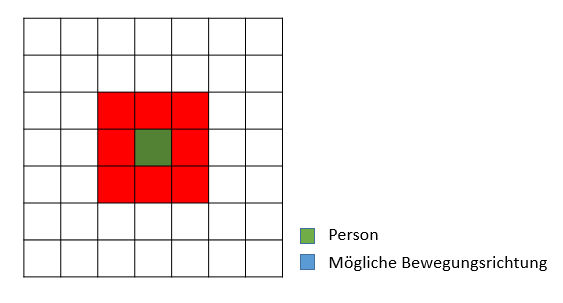
\includegraphics[width=0.5\textwidth]{abbildungen/MooreUmgebung.png}
	\caption{Moore-Umgebung}
	\label{fig:MooreUmgebung}
\end{figure}
\\
Die Personen können nur freie Zellen betreten. Jede Person wählt genau die Zelle als nächste Zelle, welche ihr den steilsten Nutzenanstieg ermöglicht. Der Nutzen der verschiedenen Zellen wird abhängig vom Betriebsmodus unterschiedlich berechnet. Darüber hinaus soll der Nutzen durch die Position der anderen Personen beeinflusst werden. \\

Hierfür wird zwischen zwei Bereichen, abhängig vom Abstand zur nächsten Person unterschieden. Beträgt der Abstand zu einer fremden Person weniger als $45cm$, wird der vertraute Bereich (intimate space) der Personen betreten. Beträgt der Abstand zwischen $45cm$ und $120cm$, wird der persönliche Bereich (personal space) der Personen betreten. Für den vertrauten Bereich ist der Nutzenverlust (Nv(x)), abhängig vom Abstand $x$, nach Funktion \ref{Equ:NutzenverlustV} definiert. Für den persönlichen Bereich wird der Nutzenverlust (Np(x)), wiederum abhängig vom Abstand $x$ zur anderen Person, durch die Funktion \ref{Equ:NutzenverlustP} definiert. 

\begin{equation}
\label{Equ:NutzenverlustP}
Np(x)= \mu * \exp(\frac{4}{(\frac{d(x)}{\delta_p * r})^{2} -1}) 
\end{equation}

\begin{equation}
\label{Equ:NutzenverlustV}
Nv(x)= Np + \frac{\mu}{a_p} * \exp(\frac{4}{(\frac{d(x)}{\delta_v * r})^{2*b_p} -1}) 
\end{equation}

$d(x)$ beschreibt den aktueller Abstand zur nächsten Person. Die folgende Tabelle enthält die Bedeutung der einzelnen Parameter und die entsprechenden Werte: 

\begin{table}[htpb]
	\centering
	\begin{tabular}{lll}
		Parameter & Beschreibung  &  Wert\\ \hline
		$\mu$ & Stärke des Nutzenverlustes & 5.0 \\
		$a_p$ & Dämpfung zwischen vertrautem und persönlichem Bereich & 1.0 \\
		$b_p$ & Stärke des Übergangs zwischen vertrautem und persönlichen Bereich &1 \\
		$\delta_p$ & persönlicher Bereich [m]& 1.20 \\
		$\delta_v$ & vertrauter Bereich [m]& 0.45 \\
		$r$ & Radius einer Person [m] & 0.2  
	\end{tabular}
	\caption{Parameter und Werte für die Berechnung des Nutzenverlustes}
	\label{tab:parameterNutzenverlust}
\end{table}

Weitere Erläuterungen zu den Parametern, den Werten und den verwendeten Funktionen sind im Kapitel \ref{Personenpotenzial} beschrieben.
 
\subsection{Geschwindigkeit der Personen}
Jede Person soll eine individuelle Wunschgeschwindigkeit besitzen. Sie bewegt sich bei freier Bahn mit dieser Geschwindigkeit fort. Die Wunschgeschwindigkeiten sollen als normalverteilt angesehen werden. Als Mittelwert und Standardabweichung sollen die errechneten Werte aus der ersten Studienarbeit verwendet werden.

\subsection{Zeitmodellierung}
Die Simulation unterliegt keinen harten Echtzeitanforderungen. Sie soll für die gesamte Simmulationsdauer so schnell wie möglich durchgeführt werden. Es soll keine globale Uhr modelliert werden. \\
Die Visualisierung der Simulation soll hingegen die Bewegungen der Personen möglichst in Echtzeit darstellen. Sie unterliegt weichen Echtzeitanforderungen. Abweichungen aufgrund mangelnder Rechner-Ressourcen sind tolerierbar. 

\subsection{Parameter}
Die Tabelle \ref{tab:parameter} zeigt alle möglichen Parameter, welche die Software steuern. Alle Parameter sind optional.
\begin{table}[htpb]
	\centering
	\begin{tabular}{lll}
		Parameter & Beschreibung  &  Default\\ \hline
		--free-flow-velocity & Mittelwert der Wunschgeschwindigkeit [m/s] & 1,0 \\
		--free-flow-deviation & Standardabweichung der Wunschgeschwindigkeiten [m/s] & 0 \\
		--algorithm & Algorithmus (euclid, dijkstra, fast-marching) & dijkstra \\
		--output-folder & Ordner in den der Output gespeichert wird & ../data/ \\
		--cellsize & Größe der einzelnen Zellen [m] & 1 \\
		--input-map & Pfad zum Bild der map (Auswahl des Testfalls) & default.png \\
		
	\end{tabular}
	\caption{Parameter und Defaultwerte}
	\label{tab:parameter}
\end{table}
	
\subsection{Berechnungen}
Die Aufgabe der Software ist die Simulation von Personenbewegungen. Für möglichst genaue Zeitangaben wird die Java Klasse BigDecimal verwendet. Für die Division werden 32 Nachkommastellen berücksichtigt und als Rundungsmodus wird Half\_Even verwendet, da dieser kumulative Fehler bei sich wiederholenden Berechnungen minimiert. Die anschließende Berechnung und Aufbereitung der Daten (insebesondere für den Test \ref{Anforderungen:RimeaTest}) erfolgt mit Mathematica.

\subsection{Report}
\label{Anforderungen:Report}
Alle errechneten Ergebnisse sollen über einen Report ausgeleitet werden.
Der Report soll im .xml Format ausgeleitet werden um eine gute Weiterverarbeitung der Ergebnisse (Visualisierung) zu gewährleisten. Die Datei $output.xml$ soll alle benötigten Informationen, wie beispielsweise die einzelnen Events der Personen, die durch den Algorithmus berechneten Entfernungen der einzelnen Zellen vom Ziel und eine Übersicht über den Zustand der einzelnen Zellen (Fieldmap), für Simulation beinhalten. \\
Die Wunschgeschwindigkeiten werden zufällig generiert. Diese sollen normalverteilt sein. Für eine Überprüfung der Zufallszahlgenerierung sollen die Wnschgeschwindigkeiten und die ID der entsprechenden Person im .csv Format in der Datei velocity.csv ausgegeben werden.

\subsection{Berechung des Zielnutzens}
\label{AnforderungenAlgorithmen}

Es sollen drei unterschiedliche Algorithmen für die Berechnung des Zielnutzens (Attraktivität) einer Zelle implementiert werden. \\
\\
Algorithmus 1: Der Nutzen bzw. die Attraktivität jeder Zelle entspricht dem negativen euklidischen Abstand. Hierbei können keine Hindernisse umgangen werden. Jede Person versucht den Nutzen zu maximieren und wählt jeweils die Zelle mit maximalen Wert aus den umliegenden aus.\\
\\
Algorithmus 2: Der Nutzen bzw. die Attraktivität jeder Zelle wird durch Floor-Flooding, basierend auf dem Dijkstra Algorithmus, berechnet. Für jede Zelle wird die geringste Anzahl an notwendigen Bewegungen bis zum Ziel ermittelt. \\
\\
Algorithmus 3: Analog zum Algorithmus 2 wird auch in diesem hier der Nutzen bzw. die Attraktivität jeder Zelle mittels Floor-Flooding berechnet. Es wird jedoch der Fast-Marching Alforithmus (Lösung der Eikonal-Gleichung) als Grundlage verwendet.

\subsection{Werte für die Auswertung}
Alle in der Tabelle \ref{tab:WerteAuswertung} aufgeführten Werte sollen auf Basis der Simulation ermittelt und ausgewertet werden. Einige Werte werden nur für bestimmte Tests benötigt.
\begin{table}[htpb]
	\centering
	\begin{tabular}{lll}
		Ermittelte Werte & Beschreibung & Wann benötigt\\ \hline
		mittlere Geschwindigkeit & durchschnittliche Geschwindigkeit der Personen im Feld & Rimea-Test 4 \\	
		Fluss (Personen/Meter/s) & Anzahl der Personen mit Geschwindigkeit > 1m/s im Feld & Rimea-Test 4\\
		Simulationsdauer & Dauer bis der Test beendet ist & Hühner Test, \\&& Evakuierung (2 Türen), \\&& Evakuierung (4 Türen)\\
	\end{tabular}
	\caption{Werte für die Auswertung}
	\label{tab:WerteAuswertung}
\end{table}

\subsection{Testszenarien für die Simulation}
\label{AnforderungenTest}

Die implementierten Algorithmen (vgl. Unterkapitel \ref{AnforderungenAlgorithmen} ) sollen anhand unterschiedlicher Testszenarien verglichen und verifiziert werden. Die verschiedenen Szenarien sollen der Simulation als .png Datei übergeben werden. 

\subsubsection{Erstellung der Testszenarien}
Es soll die Möglichkeit bestehen, unterschiedliche Testszenarien mittels eines Bildbearbeitungsprogrammes zu erstellen und an die Simulation (als .png Datei) zu übergeben. Bei der Erstellung ist sowohl die Anzahl der Personen, als auch die Anzahl der Hindernisse und Ziele (Personensenken) beliebig. Hinsichtlich der Farben der Objekte müssen jedoch die in der folgenden Tabelle \ref{tab:Farbcodes} beschriebenen Farbcodes verwendet werden. Jedes Pixel wird durch eine Zelle des Automaten repräsentiert.
 
\begin{table}[htpb]
	\centering
	\begin{tabular}{lll}
		Farbcode & Farbe & Bedeutung\\ \hline
		\#3F48CC & Blau & Ziel/ Personensenke \\	
		\#000000 & Schwarz & Ziel/ Personensenke \\
		\#FFFFFF & Weiß & Leere Zelle \\
		\#22B14C & Grün & Person 
	\end{tabular}
	\caption{Werte für die Auswertung}
	\label{tab:Farbcodes}
\end{table}
 
\subsubsection{Testszenario: Freier Fluss}
Im Zuge dieses Tests soll überprüft werden, ob sich Personen bei freier Bahn (keine Hindernisse zwischen Start und Ziel) mit ihrer jeweiligen Wunschgeschwindigkeit auf das Ziel hin bewegen. Des weiteren soll überprüft werden, ob die Person den kürzesten Weg verwendet. Der Test soll mit allen 3 Betriebsmodi durchgeführt werden. Abbildung \ref{fig:AnforderungenTest_FreierFluss} stellt den Testaufbau schematisch dar.

\begin{figure}[htpb]
	\centering
	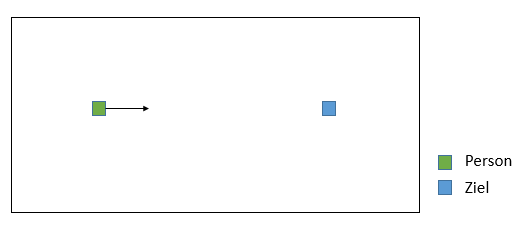
\includegraphics[width=0.8\textwidth]{abbildungen/Test_FreierFluss.png}
	\caption{Testfall Freier Fluss (schematisch)}
	\label{fig:AnforderungenTest_FreierFluss}
\end{figure}

\subsubsection{Testszenario: Hühnertest}
Zwischen Start und Ziel soll ein U-förmiges Hindernis (Öffnung in Richtung des Startes) eingefügt werden. Abhängig vom Betriebsmodus wird ein unterschiedliches Ergebnis erwartet:\\
Betriebsmodus 1: Die Personen sollen sich auf dem kürzesten Weg auf das Ziel zubewegen. Sobald sie das Hindernis erreicht haben, sollen sie stehen bleiben. Erwartungsgemäß wird der Test nicht erfolgreich verlaufen. \\
Betriebsmodi 2 und 3: Die Personen sollen das Hindernis umgehen und das Ziel erreichen. Bei einem \glqq Feststecken im Hindernis\grqq (wie im Betriebsmodus 1 gefordert) wird der Test als fehlgeschlagen gewertet. Abbildung \ref{fig:AnforderungenTest_Hühner} stellt den Testaufbau schematisch dar.

\begin{figure}[htpb]
	\centering
	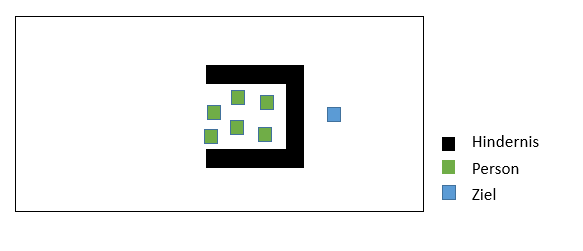
\includegraphics[width=0.8\textwidth]{abbildungen/Test_Huehner.png}
	\caption{Testfall Hühnertest (schematisch)}
	\label{fig:AnforderungenTest_Hühner}
\end{figure}
 
\subsubsection{Testszenario: Evakuierung eines Raumes mit 2 Türen}
\label{Anforderungen:Evakuierung2}
Die Personen befinden sich zu Beginn in einen von Hindernissen umgebenen, quadratischen Raum. An 2 Seiten sind Öffnungen platziert (freie Zellen). Hinter diesen Öffnungen befindet sich jeweils ein Ziel. Im Laufe des Tests sollen die Personen durch die beiden Engstellen zum Ziel gelangen. \\
Dieser Test soll mit den Betriebsmodi 2 und 3 in unterschiedlichen Versionen durchgeführt werden. Zunächst sollen sich die Türen an benachbarten Seiten befinden. Hierbei sollen sie einmal mit geringem und einmal mit sehr großem Abstand zueinander plaziert werden. Anschließend sollen die Türen an gegenüberliegenden Seiten plaziert mittig werden. Unterschiede hinsichtlich der Evakuierungsdauer sind festzuhalten. Die Abbildungen \ref{fig:AnforderungenTestEvak2TürNebeneinanderMin},  \ref{fig:AnforderungenTestEvak2TürNebeneinanderMax} und  \ref{fig:Test_Evakuierung2_Gegueb} zeigen die unterschiedlichen Testversionen schematisch.

\begin{figure}[!htb]
	\centering
	\begin{minipage}{.5\textwidth}
		\centering
		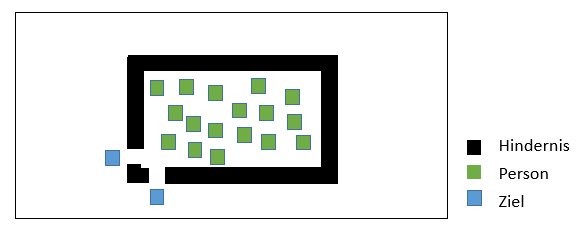
\includegraphics[width=\textwidth]{abbildungen/Test_Evakuierung2_Nebeneinander.png}
		\caption{Testfall Evakuierung eines Raumes mit 2 Türen (Nebeneinander, geringer Abstand)}
		\label{fig:AnforderungenTestEvak2TürNebeneinanderMin}
	\end{minipage}%
	\begin{minipage}{0.5\textwidth}
		\centering
		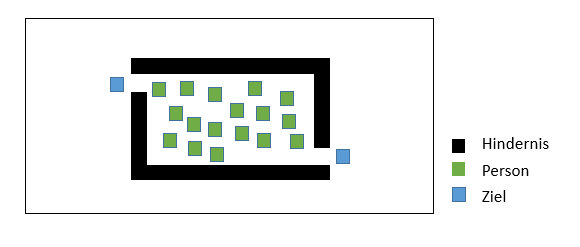
\includegraphics[width=\textwidth]{abbildungen/Test_Evakuierung2_NebeneinanderMax.png}
		\caption{Testfall Evakuierung eines Raumes mit 2 Türen (Nebeneinander, großer Abstand)}
		\label{fig:AnforderungenTestEvak2TürNebeneinanderMax}
	\end{minipage}
\end{figure}

\begin{figure}[htpb]
	\centering
	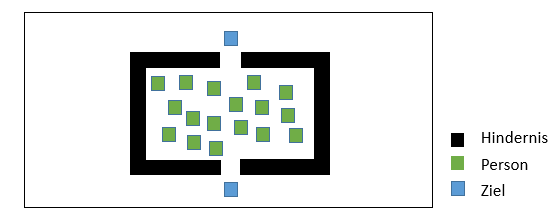
\includegraphics[width=0.8\textwidth]{abbildungen/Test_Evakuierung2_Gegueb.png}
	\caption{Testfall Evakuierung eines Raumes mit 2 Türen (Gegenüber)}
	\label{fig:Test_Evakuierung2_Gegueb}
\end{figure}

\subsubsection{Testszenario: Evakuierung eines Raumes mit 4 Türen}
Dieser Testfall entspricht der in Kapitel \ref{Anforderungen:Evakuierung2} beschriebenen Evakuierung mit 2 Türen. In diesem Fall befindet sich jedoch an jeder Raumseite eine Tür. Die Türen sollen sich in einer ersten Version mittig bezogen auf die jeweilige Raumseite befinden. Darüber hinaus sollen in einer weiteren Version die Auswirkungen ermittelt werden, wenn jeweils die 2 Türen an benachbarten Seiten mit minimalen Abstand zueinander plaziert werden. Unterschiede hinsichtlich der Evakuierungsdauer sind festzuhalten. Aufgrund der Analogie zur Evakuierung mit 2 Türen wird auf eine graphische Veranschaulichung des Testaufbaus verzichtet.

\subsubsection{Testszenario: Fundamentaldiagramm - Rimea-Test 4}
\label{Anforderungen:RimeaTest}
In diesem Testfall soll ein $65m$ langer und $12m$ breiter Gang angelegt werden. Auf der einen Seite des Ganges befindet sich die Personenquelle, auf der anderen Seite die Personensenke. Im Laufe des Testes sollen die Personen den Gang entlangschreiben. Die Anzahl der Personen ist zu variieren. In einer weiteren Version des Tests sollen Personen, welche die Personensenke erreicht haben, erneut bei der Personenquelle starten (Endlosschleife). Abbildung \ref{fig:Test_Rimea4} zeigt den Testaufbau schematisch.

\begin{figure}[htpb]
	\centering
	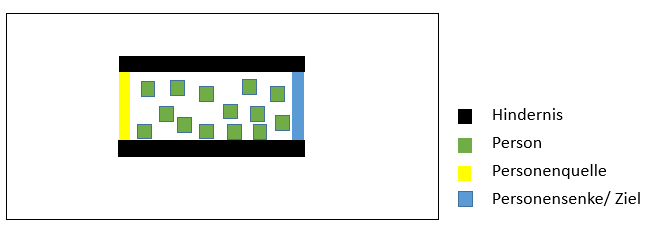
\includegraphics[width=0.8\textwidth]{abbildungen/Test_Rimea4-2.png}
	\caption{Testfall Rimea 4 (schematisch)}
	\label{fig:Test_Rimea4}
\end{figure}

\subsubsection{Testszenario: Engstelle (unidirektional)}
In diesem Testfall soll, analog zum Rimea-Test 4, ein $65m$ langer und $12m$ breiter Gang angelegt werden. Am Ende des Ganges befindet sich eine Engstelle mit $6m$ Breite und dahinter die Personensenke. Es soll mit variierender Anzahl an Personen getestet werden, wie lange es dauert bis die Engstelle durchschritten wurde. Der schematische Testaufbau ist in Abbildung \ref{fig:Engstelle} aufgeführt.

\begin{figure}[htpb]
	\centering
	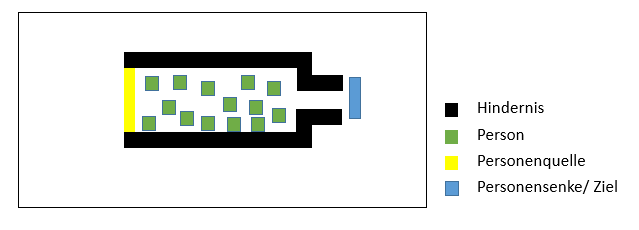
\includegraphics[width=0.8\textwidth]{abbildungen/Test_Engstelle.png}
	\caption{Testfall Engstelle (schematisch)}
	\label{fig:Engstelle}
\end{figure}

\subsection{Visualisierung}
Die Visualisierung soll die errechneten Personenbewegungen graphisch darstellen. Als Grundlage soll der ausgegebene Report (vgl. Abschnitt \ref{Anforderungen:Report}) dienen. Konkrete Anforderungen bezüglich der Visualisierung sind in Abbildung \ref{fig:AnforderungenVisualisierung} abgebildet.

\begin{figure}[htpb]
	\centering
	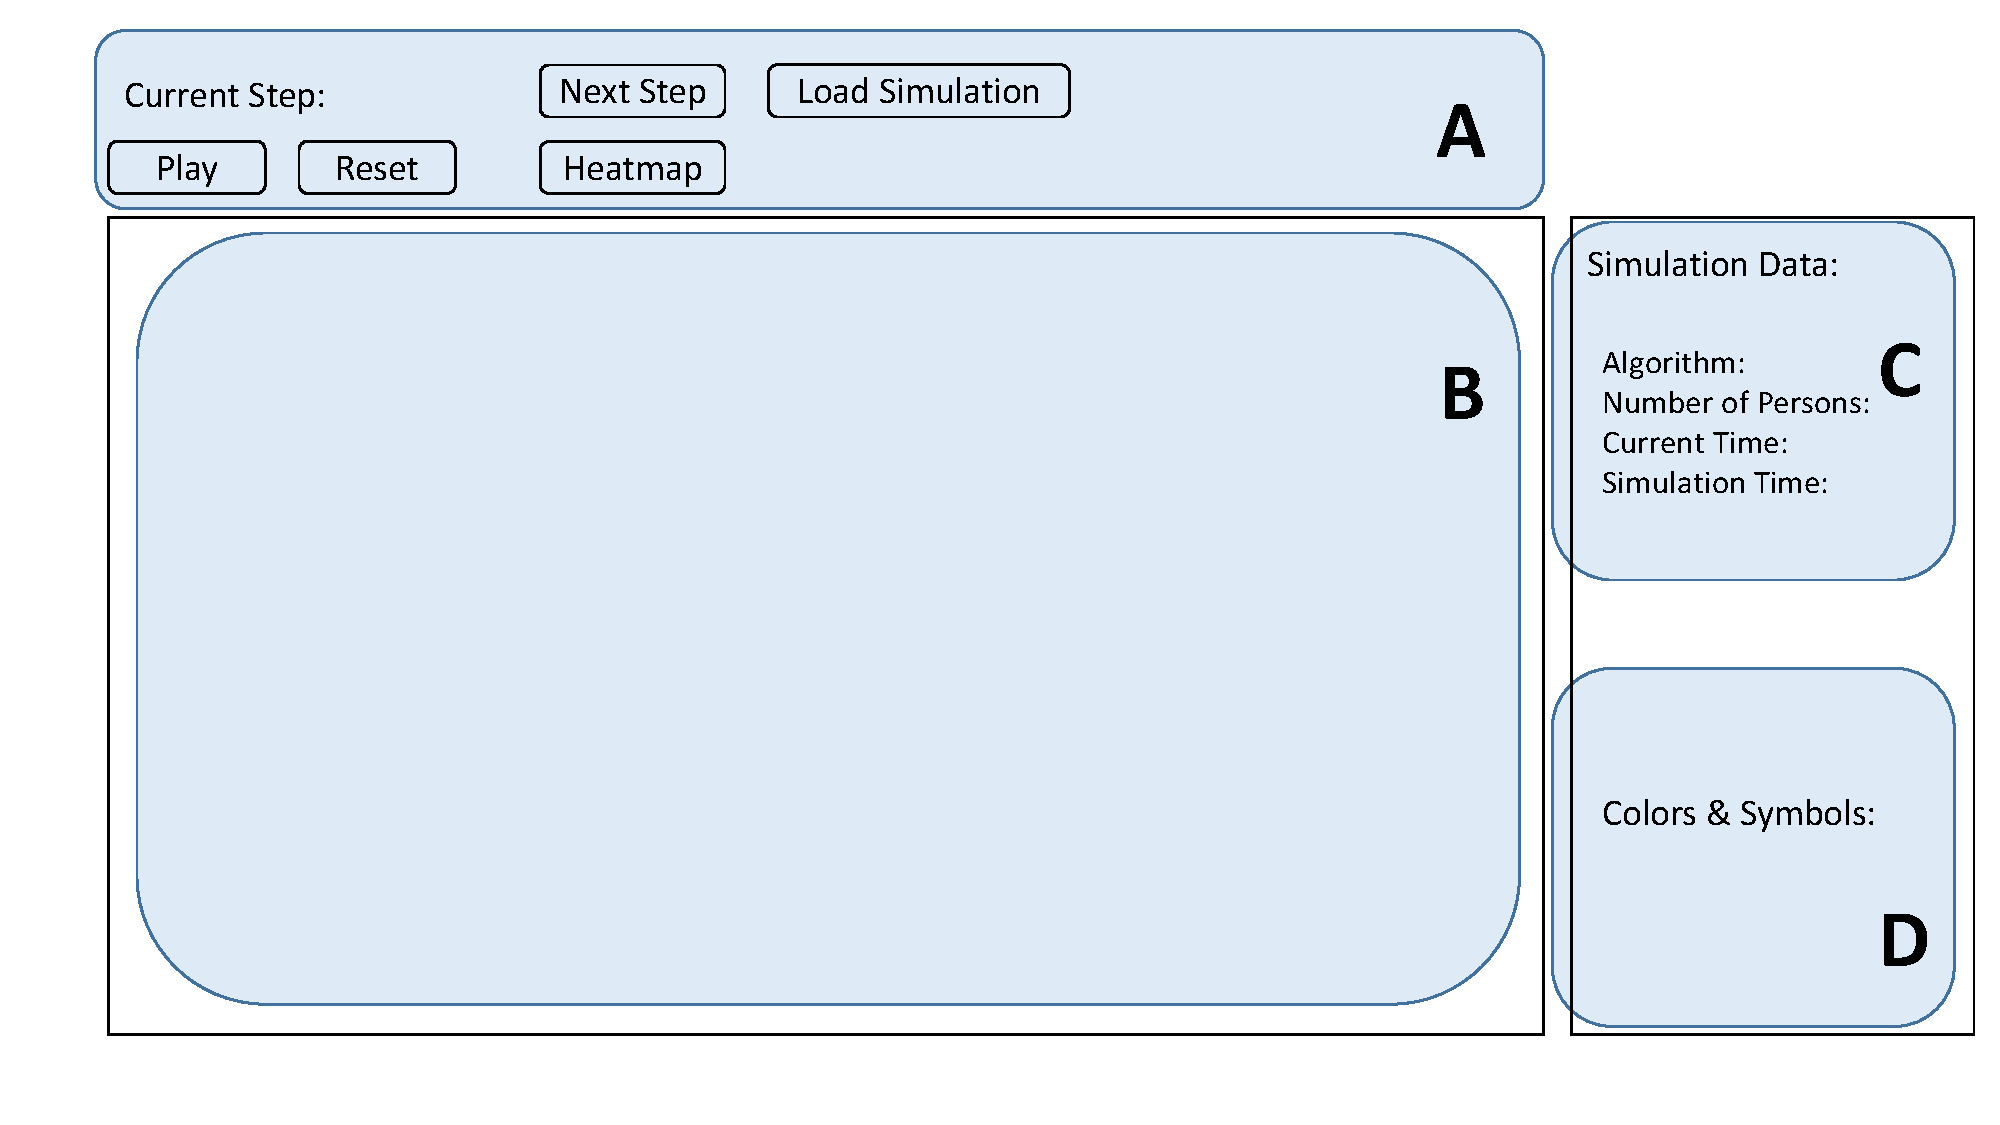
\includegraphics[width=0.8\textwidth]{abbildungen/AnforderungenVisualisierung.pdf}
	\caption{Visualisierung (schematisch)}
	\label{fig:AnforderungenVisualisierung}
\end{figure}

Die Oberfläche der Visualisierung soll aus 4 verschiedenen Teilen bestehen, welche in der Abbildung durch die blauen Kästen A-D hervorgehoben wurden. Im Teil A sollen Konfigurationsmöglichkeiten für die Visualisierung aufgeführt sein. Beispielsweise soll zwischen einer normalen Darstellung der Simulation und einer Heatmap gewechselt werden können. Darüber hinaus soll die Möglichkeit bestehen, die Visualisierung zu stoppen und schrittweise fortzusetzen. \\
Teil B enthält die eigentliche Visualisierung der Personen, Hindernisse und Ziele. In Teil C sind alle Informationen bezüglich der Visualisierung aufgeführt und Teil D enthält eine Legende der verwendeten Symbole und Farben.

\section{Softwaredesign}

Der Aufbau der Anwendung wurde im Team diskutiert und anschließend mittels UML spezifiziert.


\section{Softwaretest}


\section{Vergleich der Algorithmen}
\subsection{Euklid}
\subsection{Dijkstra}
\subsection{Fast Marching}




\section{Einfluss der Zellgröße auf die Abstandsberechnung}
Bei der Berechnung der Abstände hat die Wahl der Zellgröße je nach Algorithmus einen entscheidenden Einfluss auf die Ergebnisse der Simulation. Die Zellgröße gibt nicht nur die minimale Schrittweite vor, sondern hat auch Einfluss auf die Genauigkeit der Nutzenberechnungen. Um einen Vergleich darzustellen wurde ein Quadratisches Feld angelegt. Die Zellgröße des Feldes sowie die Anzahl der Felder wurden so variiert, dass die Entfernung von der rechten unteren Ecke zur linken oberen Ecke (am weitesten entfernter Punkt) immer den gleichen Abstand hat. Es wird also die Diagonale des Rechtecks berechnet. Die Abbildung \ref{fig_euklid_fast_marching_2m_cellsize} Zeigt den Vergleich beider Algorithmen bei der der Abstandsberechnung. Üblicherweise wird die Rabskala so gewählt um alle Werte vom kleinsten Abstand zum weitesten Punkt abzubilden. Um den Vergleich an dieser Stelle deutlich zu machen, wurde für beide Bilder die selbe Farbskala verwendet. Mit Bloßem Auge ist die Differenz nur schwer zu erkennen. Es ist jedoch sichtbar, dass das Feld, welches mit dem Euklid algorithmus berechnet wurde, einen deutlicheren Bogen aufweist. 

Eine Möglichkeit die Unterschiede zu visualisieren ist es, die Bilder mittels einer Differenzbildung der Beiden Bilder. Dafür wird ein Bild als Basis hergenommen und das zweite Bild als eine Ebene darber eingefügt. Die Farben der zweiten Ebene werden von der ersten Ebene Subtrahiert. Gleichen sich die Farben beider Ebenen, so ist das Ergebnis schwarz. Dieser Vergleich macht nur Sinn, wenn für beide Darstellungen die selbe Farbskala verwendet wurde, also die Entfernungen mit dem gleichen Farbcode codiert wurden. Die Abbildung \ref{fig_fast_marching_euclid_difference} zeigt die Differenzmenge der in Abildung \ref{fig_euklid_fast_marching_2m_cellsize} dargestellten Karten.
An diesem Bild ist deutlich zu erkennen, dass die Zellen, welche sich nur in X und nur in Y Richtung vom Ziel entfernen schwarz sind.  Es gibt also keinen Unterschied zwischen dem Euklidischen Abstand und dem Abstand welcher mittels Fast Marching berechnet wurde, bei einer Betrachtung der Zellen nur in X oder nur in Y Richtung. Entfernt man sich schräg vom Ziel (Also X und Y Anteil gleichzeitig), sieht man deutlich Differenzen der beiden Algorithmen.


Die Tabelle \ref{tab_euklid_fm_vergleich} zeigt die Ergebnisse dieses Experiments. Die Cellsize gibt dabei die Kantenlänge einer quadratischen Zelle an. Wichtig ist der Wert „Distance in X and Y“, welcher besagt, dass das Ziel in X und in Y Richtung immer jeweils 14 Zellen entfernt ist.
Nach der Formel wurde der Abstand von Ziel zum am weitesten entfernten Punkt berechnet:

$$a = \sqrt[]{x^2 +y^2} = \sqrt[]{(14\ m) ^2 +(14\ m) ^2} = 19,799\ m$$ 

Wie in der Tabelle zu sehen ist, berechnet der Euklid Algorithmus den Abstand sehr präzise. Da der Euklid Algorithmus kein „Gedächtnis“ hat also ohne Einfluss vorheriger Zellen berechnet und die oben genannte Formel anwendet ist der Algorithmus gut geeignet um die exakte Entfernung zu berechnen. Interessant in der Tabelle ist vor allem die Abweichung von 1,45 m, welche beim Fast Marching Algorithmus entsteht. Diese Abweichung entspricht einem Fehler von von 7,3 \% bezogen auf die tatsächliche Entfernung. Verringert man die Zellgröße, so konvergiert der Fast Marching Algorithmus gegen den euklidischen Abstand und der Fehler gegen 0. Die prozentualen Fehler in Abhängigkeit der Zellgröße sind in Abbildung \ref{fig_fast_marching_error_cellsize} dargestellt. 

\section{Einfluss der Zellgröße auf die maximale Dichte}
Darüber hinaus hat die Zellgröße direkten Einfluss auf die Dichte [$\frac{Personen}{m^2}$] in einem Feld. Würde man die Zellgröße von $2\ m^2$ wählen, erhielte man eine maximale Dichte von 0,5 $\frac{1}{m^2}$. Es ist darauf zu achten, dass die Zellgröße angemessen gewählt wird. Bei weiteren Versuchen wurde stets eine Zellbreite von 0,4 bis 0,5 m verwendet, sofern nichts anderes angegeben.



\begin{figure}
\centering
\begin{minipage}{.44\textwidth}
\centering
  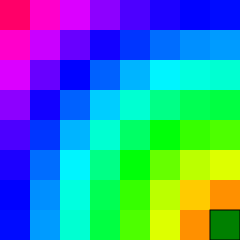
\includegraphics[width=0.9\linewidth]{abbildungen/vergleich_euklid_fast_marching/eEuclid_2m.png}
\end{minipage}%
\begin{minipage}{.44\textwidth}
\centering
  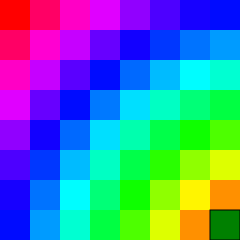
\includegraphics[width=0.9\linewidth]{abbildungen/vergleich_euklid_fast_marching/eFastMarching_2m.png}
\end{minipage}
\begin{minipage}{.1\textwidth}
\centering
  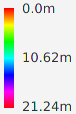
\includegraphics[width=\linewidth]{abbildungen/vergleich_euklid_fast_marching/farbskala.png}
\end{minipage}
\caption{Berechnung der Abstände mittels Euklid (links) und Fast Marching (rechts) an einem Feld mit einer Zellbreite von 2\ m. Dunkelgrün: Ziel, Rot: am weitesten entfernter Punkt im Feld}
\label{fig_euklid_fast_marching_2m_cellsize}
\end{figure}



\begin{figure}[ht]
	\centering
  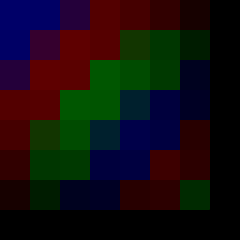
\includegraphics[width=0.4\textwidth]{abbildungen/vergleich_euklid_fast_marching/differenz_euklid_fast_marching.png}
	\caption{Differenzbildung der beiden Karten Euklid und Fast Marching}
	\label{fig_fast_marching_euclid_difference}
\end{figure}



\begin{table}[htbp]
\begin{tabular}{|l|r|r|r|r|r|r|r|}
\hline
Cellsize [m] & 2 & 1 & 0,5 & 0,25 & 0,125 & 0,0625 & 0,03125 \\ \hline
Cells in X and Y & 7 & 14 & 28 & 56 & 112 & 224 & 448 \\ \hline
Distance in  & & &  & &  & &\\ X and Y [m] & \textbf{14} & \textbf{14} & \textbf{14} & \textbf{14} & \textbf{14} & \textbf{14} & \textbf{14} \\ \hline
Tatsächliche & & &  & &  & &\\Entfernung [m] & 19,799 & 19,799 & 19,799 & 19,799 & 19,799 & 19,799 & 19,799 \\ \hline
Euklid [m] & 19,799 & 19,799 & 19,799 & 19,799 & 19,799 & 19,799 & 19,799 \\ \hline
Fast  & & &  & &  & &\\ Marching [m] & \textbf{21,245} & \textbf{20,717} & \textbf{20,363} & \textbf{20,137} & \textbf{19,997} & \textbf{19,913} & \textbf{19,863} \\ \hline
Diff [m] & 1,45 & 0,92 & 0,5645 & 0,3380 & 0,1979 & 0,1138 & 0,0644 \\ \hline
 & \multicolumn{1}{l|}{} & \multicolumn{1}{l|}{} & \multicolumn{1}{l|}{} & \multicolumn{1}{l|}{} & \multicolumn{1}{l|}{} & \multicolumn{1}{l|}{} & \multicolumn{1}{l|}{} \\ \hline
Error [\%]  & & &  & &  & &\\ diff/distance & \textbf{7,30} & \textbf{4,64} & \textbf{2,85} & \textbf{1,71} & \textbf{1,00} & \textbf{0,57} & \textbf{0,33} \\ \hline
\end{tabular}
\caption{Vergleich der Algorithmen Fast Marching und Euklid. Cellsize ist die Kantenlänge einer quadratischen Zelle in m (Zellbreite)}
\label{tab_euklid_fm_vergleich}
\end{table}


\begin{figure}[ht]
	\centering
  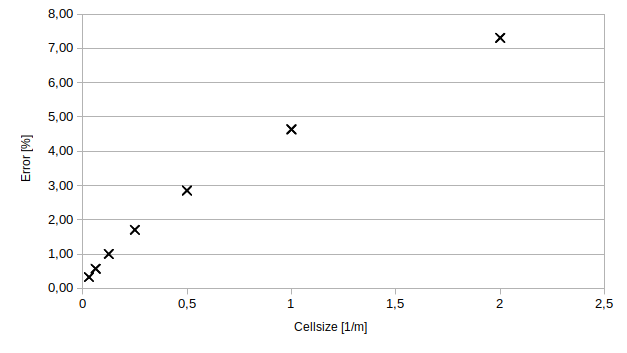
\includegraphics[width=\textwidth]{abbildungen/vergleich_euklid_fast_marching/fehler_zellgroesse.png}
	\caption{Prozentualer Fehler des Fast Marching Algorithmus in Abhängigkeit der Zellbreite}
	\label{fig_fast_marching_error_cellsize}
\end{figure}





\subsection{Verifikation}

\subsubsection{Evakuierung}
Mit Hilfe der verschiedenen Evakuierungstests sollen die Auswirkungen unterschiedlicher Positionen und Anzahl von Türen auf die Dauer der Evakuierung eines Raumes ermittelt werden. Die Berechnung des Zielnutzens auf Basis des Euklid Algorithmus wird hierbei nicht berücksichtigt. Dieser Algorithmus ist zwar gut geeignet um den kürzesten Weg zu einem Ziel zu finden, Hindernisse können jedoch nicht umgangen werden. Somit kann nicht ausgeschlossen werden, dass eine Person, beispielsweise in einer Ecke, \glqq hängen bleibt\grqq. Dieses Verhalten würde nicht der Realität entsprechen.

\paragraph{Evakuierung eines Raumes (Personen befinden sich in der Mitte)}
\label{EvaVerifikation}
Für die Verifikation der Simulation sollen sich die Personen zunächst alle dicht gedrängt in der Mitte des Raumes befinden. An 2 gegenüberliegenden Seiten des Raumes soll sich jeweils eine Tür befinden (Evakuierung eines Raumes mit 2 Türen). In einer weiteren Simulation sollen sich an den anderen beiden Seiten jeweils eine weitere Tür befinden (Evakuierung eines Raumes mit 4 Türen). Die Evakuierungsdauer des Raumes mit 4 Türen müsste nun exakt halb so lange sein, wie die des Raumes mit 2 Türen. \\ 

\paragraph{Evakuierung eines Raumes (Personen zufällig verteilt)}
Das in Abschnitt \ref{EvaVerifikation} beschriebene Szenario ist zwar für die Verifikation der Simulation relevant, in der Realität jedoch äußerst unwahrscheinlich. Die Personen in einem Raum werden sich nie dicht gedrängt, exakt symmetrisch in der Mitte befinden. Aus diesem Grund werden in diesem Abschnitt weitere Evakuierungstests gegenübergestellt, bei denen die Personen zufällig im Raum verteilt wurden. Anhand dieser Tests sollen die Auswirkungen unterschiedlicher Positionen und Anzahl der Türen auf die Evakuierungsdauer simuliert werden.\\

\begin{figure}[htpb]
	\centering
	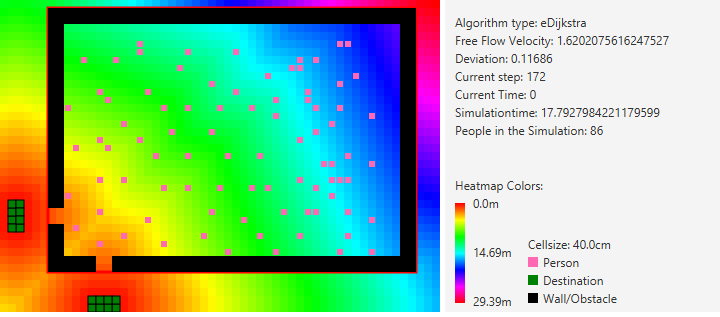
\includegraphics[width=0.8\textwidth]{abbildungen/Evak1DBegin.png}
	\caption{Verteilung der Personen (Heatmap Dijkstra Algorithmus)}
	\label{fig:EvakuierungMap}
\end{figure}

Abbildung \ref{fig:EvakuierungMap} zeigt die Verteilung der Personen, die für alle weiteren Evakuierungstests in diesem Kapitel verwendet werden. Somit wird eine bessere Vergleichbarkeit der Ergebnisse erzielt. In der Abbildung ist außerdem die Heatmap des Dijkstra Algorithmus für dieses Szenario zu sehen. 

\begin{figure}[!htb]
	\centering
	\begin{minipage}{.5\textwidth}
		\centering
		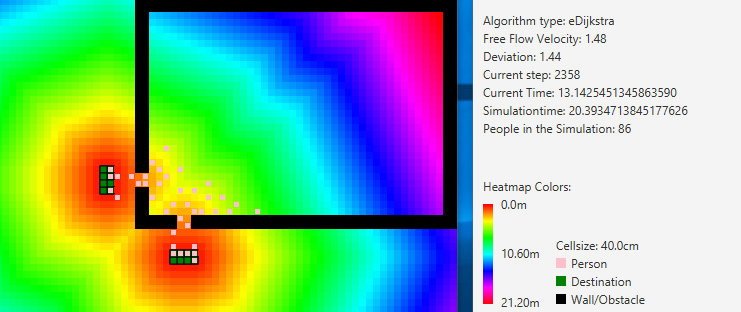
\includegraphics[width=\textwidth]{abbildungen/Evak1DMitte.png}
		\caption{Evakuierung eines Raumes mit 2 Türen (geringer Abstand, Dijkstra Algorithmus)}
		\label{fig:Evak2TürNebeneinanderMinDijkstra}
	\end{minipage}%
	\begin{minipage}{0.5\textwidth}
		\centering
		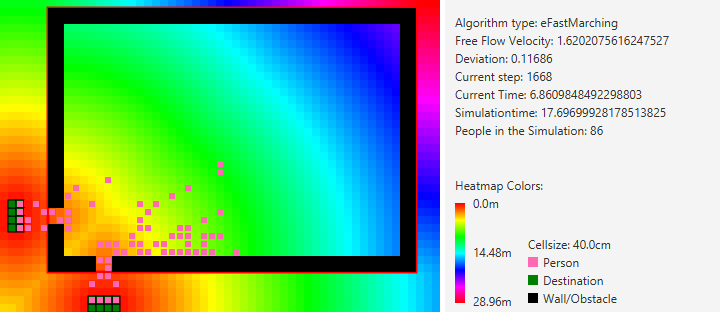
\includegraphics[width=\textwidth]{abbildungen/Evak1FMMitte.png}
		\caption{Evakuierung eines Raumes mit 2 Türen (geringer Abstand, Fast Marching Algorithmus)}
		\label{fig:Evak2TürNebeneinanderMinFM}
	\end{minipage}
\end{figure}

Die Abbildungen \ref{fig:Evak2TürNebeneinanderMinDijkstra} und \ref{fig:Evak2TürNebeneinanderMinFM} zeigen einen Ausschnitt der Simulation nach einer Simulationszeit von ca. $13s$. Wie zu erwarten ist, drängen alle Personen in die Ecke links unten. Dort bilden sich vor den Engstellen (Ausgängen) kleinere Staus. Die Evakuierungsdauer beträgt für die Simulation mit dem Dijkstra Algorithmus ca. $20s$. Da sich die Personen bei Verwendung des Fast Marching Algorithmus effizienter auf die Ziele zu bewegen, bilden sich etwas kleinere Staus an den Engstellen und die Evakuierungsdauer ist mit ca. $18,7s$ etwas kürzer.

\begin{figure}[!htb]
	\centering
	\begin{minipage}{.5\textwidth}
		\centering
		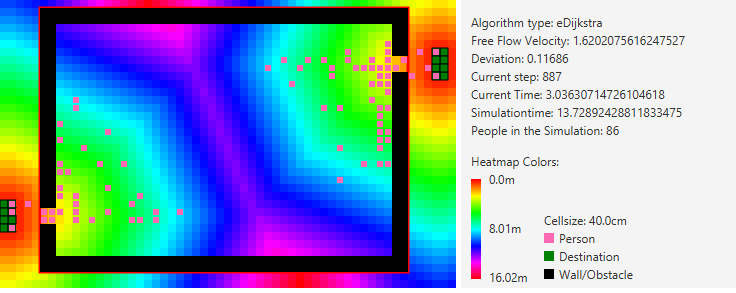
\includegraphics[width=\textwidth]{abbildungen/Evak2DMitte.png}
		\caption{Evakuierung eines Raumes mit 2 Türen (großer Abstand, Dijkstra Algorithmus)}
		\label{fig:Evak2TürNebeneinanderMaxDijkstra}
	\end{minipage}%
	\begin{minipage}{0.5\textwidth}
		\centering
		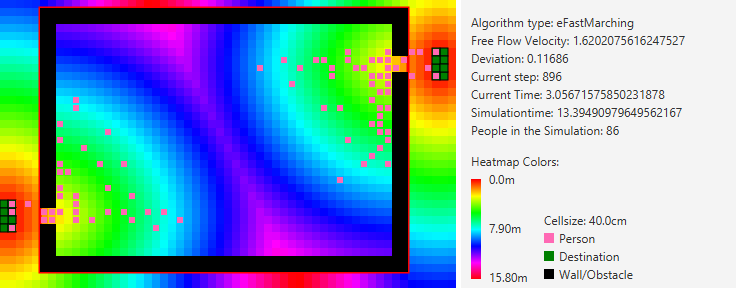
\includegraphics[width=\textwidth]{abbildungen/Evak2FMMitte.png}
		\caption{Evakuierung eines Raumes mit 2 Türen (großer Abstand, Fast Marching Algorithmus)}
		\label{fig:Evak2TürNebeneinanderMaxFM}
	\end{minipage}
\end{figure}

Im Vergleich dazu zeigen die Abbildungen \ref{fig:Evak2TürNebeneinanderMaxDijkstra} und \ref{fig:Evak2TürNebeneinanderMaxFM} jeweils einen Ausschnitt einer Simulation, in der die Ausgänge bzw. Ziele sehr weit voneinander entfernt gewählt wurden. In beiden Abbildungen ist sofort zu sehen, dass sich in etwa die Hälfte der Personen (Personen deren Startposition in der entsprechenden Hälfte lag) auf die Ziele unten links und die andere Hälfte auf die Ziele oben rechts zubewegen. Die Heatmaps zeigen die entsprechende Entfernung an. Die maximale Entfernung vom Ziel ist mit ca. $16m$ deutlich geringer als in der eben beschriebenen Simulation ($21m$). Die bessere Verteilung der Personen auf die Ziele und die geringere Entfernung zum Ziel erklären die geringer Evakuierungsdauer von ca. $19,5s$ (Dijkstra) bzw. $18,5s$ (Fast-Marching).
%TODO: Noch ne SImulation mit mehr Personen um Unterschied zu verdeutlichen
\paragraph{Fazit und Vergleich}

\subsection{Validation}

\section{Ausblick und Fazit}

%----------------------------------------------------------------------------------------
%\input{References}
\bibliography{Bibliographie}
\bibliographystyle{plain}

\end{document}
